\newpage 

\section{Memory Hierarchy Optimizations}

Software-controlled data prefetching is a promising technique for
improving the performance of the memory subsystem to match
today’s high-performance processors. While prefctching is useful in
hiding the latency, issuing prefetches incurs an instruction overhead
and can increase the load on the memory subsystem. As a resu 1~
care must be taken to ensure that such overheads do not exceed the
benefits.


\subsection{Introduction}

Various hardware and software approaches to improve the memory
performance have been proposed recently [15]. A promising technique 
to mitigate the impact of long cache miss penalties is softwarecontrolled
 prefetching[5, 13, 16, 22 23]. Software-controlled
prefetching requires support from both hardware and software. The
processor must provide a special “prefetch” instruction. The software 
uses this instruction to inform the hardware of its intent
to use a particular data item, if the data is not cumently in the
cache, the data is fetched in from memory. The cache must be
lockup-free[17]; that is, the cache must allow multiple outstrmding
 misses. While the memory services the data miss, the program
can continue to execute as long as it does not need the requested
data. While prefetching does not reduce the latency of the memory
access, it hides the memory latency by overlapping the access with
computation and other accesses. Prefetches on a scalar machine
are analogous to vector memory accesses on a vector machine. In
both cases, memory accesses are overlapped with computation and
other accesses. Furthermore, similar to vector registers, prefetching
allows caches in scalar machines to be managed by software. A
major difference is that while vedor machines can only operate on
vectors in a pipelined manner, scalar machines can execute arbitrary
sets of scalar operations well.


Another useful memory hierarchy optimization is to improve data
locality by reordering the execution of iterations. One important
example of such a transform is blocking[l, 9, 10, lZ 21, 23, 29].
Instead of operating on entire rows or columns of an array, blocked
algorithms operate on submatrices or blocks, so that datu loaded
into the faster levels of the memory hkmarchy are reused. Other
useful transformations include unimodular loop transforms such as
interchange, skewing and reversal[29]. Since these optimization
improve the @de’s data locality, they not only reduee the effeetive
 memory access time but also reduce the memory bandwidth
requirement. Memory hierarchy optimization such as prefetching
and blocking are crucial to turn high-performance microprocessors
into effective scientific engines.



\subsection{Blocking\cite{lam1991cache}}


Blocking is a well-known optimization technique for improving
the effectiveness of memory hierarchies. Instead of operating on
entire rows or columns of an array, blocked algorithms operate on
submatrices or blocks, so that data loaded into the faster levels
of the memory hierarchy are reused. This paper presents cache
performance data for blocked programs and evaluates several optimization 
to improve this performance. The data is obtained by
a theoretical model of data conflicts in the cache, which has been
validated by large amounts of simulation.

Due to high level integration and superscalar architectural designs,
the floating-point arithmetic capability of microprocessors has increased significantly in the last few years. Unfortunately, the increase in processor speed has not been accompanied by a similar
increase in memory speed. To fully realize the potential of the
processors, the memory hierarchy must be efficiently utilized.

While data caches have been demonstrated to be effective for
general-purpose applications in bridging the processor and memory speeds, their effectiveness for numerical code has not been
established. A distinct chmactenstic of numerical applications is
that they tend to operate on large data sets. A cache may only be
able to hold a small fraction of a matrix; thus even if the data are
reused, they may have been displaced from the cache by the time
they are reused.

Consider the example of matrix multiplication for matrices of size
NxN:

\begin{figure}[H]
	\centering
	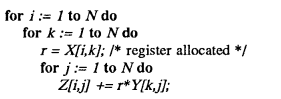
\includegraphics[width=0.6\textwidth]{p194.png}
	\caption{matrix multiplication example}
	\label{fig:p194}
\end{figure}



Figure \ref{fig:p193}(a) shows the data access pattern of this code. The same
element $X[i,k]$ is used by all iterations of the innermost loop; it
can be register allocated and is fetched from memory only once.
Assuming that the matrix is organized in row major order, the
innermost loop of this code accesses consecutive data in the Y
and $Z$ matrices, and thus utilizes the cache prefetch mechanism
fully. The same row of $Z$ accessed in an innermost loop is reused
in the next iteration of the middle loop, and the same row of
$Y$ is reused in the otftermost loop. Whether the data remains in
the cache at the time of reuse depends on the size of the cache.
Unless the cache is large enough to hold at least one $N * N$
matrix, the data Y would have been displaced before reuse. If
the cache cannot hold even one row of the data then $Z$ data in
the cache cannot be reused. In the worst case, $2N^3 + N^2$ words
of data need to be read from memory in $N^3$ iterations. The high
ratio of memory fetches to numerical operations can significantly
slow down the machine.


\begin{figure}[H]
	\centering
	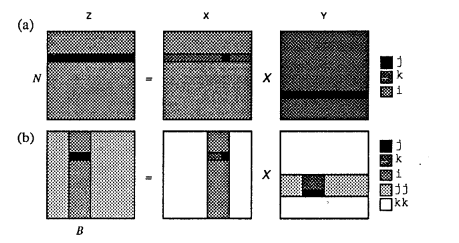
\includegraphics[width=0.6\textwidth]{p193.png}
	\caption{Data access pattern in (a) unblocked and (b) blocked matrix multiplication.}
	\label{fig:p193}
\end{figure}


It is well known that the memory hierarchy can be better 
utilized if scientific algorithms are blocked.
Blocking is also known as tiling. 
Instead of operating on individual matrix entries, 
the calculation is performed on submatrices.


Blocking can be applied to any and multiple levels of memory
hierarchy, including virtual memory, caches, vector registers, and
scalar registers. The matrix multiplication code
blocked to reduce cache misses looks like this:

\begin{figure}[H]
	\centering
	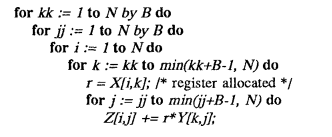
\includegraphics[width=0.6\textwidth]{p195.png}
	\caption{Reduced matrix multiplication example.}
	\label{fig:p195}
\end{figure}


Figure \ref{fig:p193}(b) shows the data access pattern of the 
blocked code. We
observe that the original data access pattern is reproduced here,
but at a smaller scale. The blocking factor, $B$ , is chosen so that
the $B * B$ submatrix of $Y$ and a row of length $B$ of $Z$ can fit in
the cache. In this way, both $Y$ and $Z$ are reused $B$ times each time
the data rue brought in. Thus, the total memory words accessed
is $2N^3/B + N2$ if there is no interference in the cache.

Blocking is a general optimization technique for increasing the
effectiveness of a memory hierarchy. By reusing data in the faster
level of the hierarchy, it cuts down the average access latency.
It also reduces the number of references made to slower levels
of the hierarchy. Blocking is thus superior to optimization such
us prefetching, which hides the latency but does not reduce the
memory bandwidth requirement. This reduction is especially important for multiprocessors since memory bandwidth is often the
bottleneck of the system.

